%   % !TEX root = ../../VIII,3_Rahmen-TeX_9-0.tex
%  
%   Signatur/Tex-Datei:	LH_37_05_157-158
%   RK-Nr. 	57270
%				
%   Überschrift: 	Certa de motu
%   Datierung:		10. (20.) Juni 1677 (eigh.)
%   edlabels:			5	
%   Diagramme: 		2
%
%
\selectlanguage{ngerman}
\frenchspacing
%
\begin{ledgroupsized}[r]{120mm}
\footnotesize
\pstart
\noindent\textbf{Überlieferung:}
\pend
\end{ledgroupsized}
%
\begin{ledgroupsized}[r]{114mm}
\footnotesize
\pstart \parindent -6mm
\makebox[6mm][l]{\textit{L}}%
Konzept:
LH~XXXVII~5, Bl.~157\textendash158. 
Ein Bogen~4\textsuperscript{o}; Wasserzeichen im Falz; Ränder beschnitten; Papiererhaltungsmaßnahmen.
Vier Seiten.
%Diverses.
\pend
\end{ledgroupsized}
%
\begin{ledgroupsized}[r]{114mm}
\footnotesize
\pstart
\parindent -6mm
\makebox[6mm][l]{\textit{E}}%
\textsc{Fichant} 1994, S.~379\textendash383\cite{01056}.\pend%
\end{ledgroupsized}
%
%
\vspace{5mm}
\begin{ledgroup}
\footnotesize
\pstart
\noindent%
\textbf{Datierungsgründe:}	
Sowohl das vorliegende Konzept als auch N.~\ref{RK57269} sind eigh.\ auf den 10.\ (20.) Juni 1677 datiert.
%
Leibnizens Analyse des Stoßes in N.~\ref{RK57270} bezieht sich ausdrücklich auf die Schiffsanalogie
%
(siehe bspw.\ S.~\refpassage{37_05_157-158_5a}{37_05_157-158_5b}).
%
Diese wird aber in N.~\ref{RK57270} nicht eigens eingeführt, sondern vorausgesetzt,
%
wohingegen der Großteil von N.~\ref{RK57269} einer ausführlichen Besprechung derselben gewidmet ist.
%
Dieser Umstand lässt auf die spätere Entstehung von N.~\ref{RK57270} gegenüber N.~\ref{RK57269} schließen.
%
\pend 
\end{ledgroup}
%
%
\selectlanguage{latin}
\frenchspacing
% \newpage%
\vspace{8mm}
\pstart%
\normalsize%
\noindent%
\lbrack157~r\textsuperscript{o}\rbrack\
\pend
\count\Bfootins=1100%
\count\Afootins=1100%
\count\Cfootins=1100
%
\pstart
\raggedleft
10 Jun.\ 1677
\pend 
%
\pstart
\centering
Certa de motu.%
\protect\index{Sachverzeichnis}{motus}
\pend
\vspace{0.5em}
\pstart
1.\ Corpora eandem semper servant potentiam\protect\index{Sachverzeichnis}{potentia}. 
\pend \pstart
2.\ Si duo \edtext{corpora sibi occurrant}{\lemma{corpora}\Bfootnote{\textit{(1)}~concurrant \textit{(2)}~sibi occurrant~\textit{L}}} celeritatibus reciproce proportionalibus%
\protect\index{Sachverzeichnis}{celeritates reciproce proportionales}
recurrent ambo eadem celeritate qua venere.
\pend \pstart
3.\ Si corpus incurrat in quiescens immobile,%
\protect\index{Sachverzeichnis}{corpus quiescens immobile}%
\protect\index{Sachverzeichnis}{incursus corporis in quiescens immobile} recurret ea qua 
venit celeritate.
\pend 
\pstart
4.\ Si corpus incurrat in corpus 
%
\edtext{quod repellere}{\lemma{quod}\Bfootnote{\textit{(1)}~propellere \textit{(2)}~repellere~\textit{L}}} non possit, recurret sua celeritate.
Quod ita intelligo:
\pend
%
\vspace{1.5em} %%%%%%%%% Diagramm 1
\centerline{%
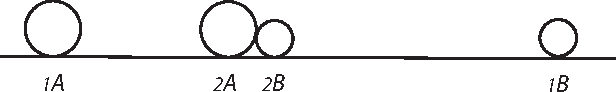
\includegraphics[width=0.75\textwidth]{%
gesamttex/edit_VIII,3/images/LH_37_05_157-158_d1_157r.pdf%
}} 
\vspace{0.5em}
\centerline{%
\lbrack\textit{Fig.~1}\rbrack%
}
% \newpage%
\vspace{1.5em}
%
\pstart
Ponamus \edtext{corpus \textit{B}}{\lemma{corpus}\Bfootnote{\textit{(1)}~\textit{A} \textit{(2)}~\textit{B}~\textit{L}}}
%
incurrere in corpus \textit{A}, sed ipsum
non posse repellere, quia alterum est fortius,%
\protect\index{Sachverzeichnis}{corpus fortius} tunc 
si repellere non potest, sive si ei non potest communicare
aliquem conatum retrorsum,%
\protect\index{Sachverzeichnis}{conatus retrorsus} necesse est ut ipsum retrorsum 
tendat eo conatu, quem alteri commu-
\pend
\newpage
\pstart
\noindent nicare debuerat,
nam si alterum nonnihil retroageret, conatu%
\protect\index{Sachverzeichnis}{conatus} scilicet quem ei impingit\lbrack,\rbrack\
tunc altero simul progrediente
et redeunte, utique progrederetur reapse %
differentia progressus et regressus\protect\index{Sachverzeichnis}{differentia progressus et regressus}, et ita perdita fuisset 
%
\edtext{potentia\protect\index{Sachverzeichnis}{potentia}, neque}{\lemma{potentia,}\Bfootnote{\textit{(1)}~itaque cum \textit{(2)}~neque~\textit{L}}} 
%
vero fingi potest hanc potentiam\protect\index{Sachverzeichnis}{potentia} corpori obstanti communicare, ad
%
\edtext{pergendum uti}{\lemma{pergendum}\Bfootnote{\textit{(1)}~in contrariam, necesse est \textit{(2)}~uti~\textit{L}}}
%
venit, necesse est ergo %
corpus debilius\protect\index{Sachverzeichnis}{corpus debilius} quod impegit 
in fortius%
\protect\index{Sachverzeichnis}{corpus fortius} tota sua potentia\protect\index{Sachverzeichnis}{potentia} 
%
\edtext{retroire. Superest}{\lemma{retroire}\Bfootnote{\textit{(1)}~, fortius autem \textit{(2)}~. Superest~\textit{L}}} 
%
tantum ut quaeramus
\edtext{an fortius\protect\index{Sachverzeichnis}{corpus fortius} tota}{\lemma{an fortius}\Bfootnote{\textit{(1)}~sua \textit{(2)}~tota~\textit{L}}} 
%
sua potentia\protect\index{Sachverzeichnis}{potentia} pergat, an vero ejus nonnihil communicet
debiliori\protect\index{Sachverzeichnis}{corpus debilius} ad augendum ejus 
%
\edtext{recursum.%
\protect\index{Sachverzeichnis}{recursus} Eo momento}{\lemma{recursum.}\Bfootnote{\textit{(1)}~Et quidem eo momento quo agit in fortius, utique \textit{(a)}~ei dat conatum redeundi \textit{(b)}~conatus est in tota massa composita ex fortiore et potentiore, isque \textit{(2)}~Eo momento quo \textit{(a)}~corpus \textit{(b)}~corpora~\textit{L}}} 
%
quo corpora \textit{A} et \textit{B} sibi 
%
\edtext{occurrunt tunc}{\lemma{occurrunt}\Bfootnote{\textit{(1)}~tunc massa tota $A+B$ \textit{(2)}~tunc~\textit{L}\hspace{-2mm}}} 
%
corpus \textit{{\scriptsize 2}A} fortius%
\protect\index{Sachverzeichnis}{corpus fortius} ipsi \textit{{\scriptsize 2}B} debiliori communicat conatum
aliquem, eundi%
\protect\index{Sachverzeichnis}{conatus eundi} versus \textit{{\scriptsize 1}B}, nimirum talem,
%
\edtext{ut}{%
\lemma{}%
\Bfootnote{%
ut %
\textit{gestr.~L, wieder gültig gemacht Hrsg.}%
}}
%
\edtext{ips\lbrack um\rbrack}{%
\lemma{}%
\Bfootnote{%
ipsa %
\textit{L ändert Hrsg.}%
}}
%
sibi de potentia\protect\index{Sachverzeichnis}{potentia eundi} eodem eundi retineat 
partem magnitudini suae proportionalem, 
%
\edtext{itaque perget}{\lemma{itaque}\Bfootnote{\textit{(1)}~illuc ibit \textit{(2)}~perget~\textit{L}}} 
%
corpus \edtext{\textit{A} minore}{\lemma{\textit{A}}\Bfootnote{\textit{(1)}~celeritate minore qua \textit{(2)}~minore~\textit{L}}} 
%
quam ante celeritate, recurret corpus \textit{B} majore.
%
\pend
%
\pstart
Unum tantum examinandum est, ponamus corpus \textit{{\scriptsize 2}A}, postquam ipsi \textit{{\scriptsize 2}B}, conatum redeundi%
\protect\index{Sachverzeichnis}{conatus redeundi} 
dedit, fieri debilius ipso \textit{{\scriptsize 2}B}, vel etiam tunc aequalem habere potentiam\protect\index{Sachverzeichnis}{potentia} cum potentia\protect\index{Sachverzeichnis}{potentia} 
ipsius \textit{{\scriptsize 2}B}, cum ipsi \textit{{\scriptsize 2}B} suam dedit, sed quia tunc considerandum est, etiam ipsum \textit{{\scriptsize 2}B} potentiam\protect\index{Sachverzeichnis}{potentia} exiguam retinuisse, post conatum quem alteri dedit, ideo res eo redibit, 
ut hoc consideremus: corpus \textit{A}, accepit a corpore 
%
\edtext{\textit{B} potentiam\protect\index{Sachverzeichnis}{potentia}}{\lemma{\textit{B}}\Bfootnote{\textit{(1)}~potentiam eundi \textit{(2)}~impetum (\protect\vphantom)impetus est ad conatum, ut conatum \textit{(3)}~potentiam~\textit{L}}} 
%
eundi%
\protect\index{Sachverzeichnis}{potentia eundi} in eas partes ad quas tendit \textit{B}, quae sit ad potentiam\protect\index{Sachverzeichnis}{potentia} qua venit \textit{B}, ut \textit{A} ad $A+B$, et 
%
\edtext{alterum \textit{B}}{\lemma{}\Bfootnote{alterum \textbar\ vicissim \textit{gestr.}\ \textbar\ \textit{B}~\textit{L}}} 
%
ab \edtext{\textit{A}. Duae}{\lemma{\textit{A}.}\Bfootnote{\textit{(1)}~Si jam \textit{(2)}~Duae~\textit{L}}} 
%
ergo sunt in \textit{B} potentiae\lbrack,\rbrack\protect\index{Sachverzeichnis}{potentia} 
una eundi%
\protect\index{Sachverzeichnis}{potentia eundi} in unam altera in alteram partem, ex quibus vincet major. Quaeritur jam 
an major sine contradictione vincat excessu, differentia vero \edtext{potentiae\protect\index{Sachverzeichnis}{differentia potentiae}}{\lemma{potentiae}\Bfootnote{\textit{erg.}~\textit{L}}}, 
ita distribuatur, ut 
%
\edtext{ipsa quia}{\lemma{ipsa}\Bfootnote{\textit{(1)}~pro rata
\textit{(a)}~inter
\textit{(b)}~detur
\textit{(2)}~quia~\textit{L}}} 
%
perdi non debet aequaliter detur uni corpori atque alteri, in diversas
scilicet partes. An vero major suum exequitur sine diminutione, minore quae nihil
efficere potest, alteri reddita quod dedit. Si ponimus excessu tantum agere,
%
% 	====== end of 157 r ==
%
\lbrack157~v\textsuperscript{o}\rbrack\
et differentiam%
\protect\index{Sachverzeichnis}{differentia potentiae} redhiberi, tunc in eo quod differentiam recipit idem
continget, et dabitur nova %
redhibitio\protect\index{Sachverzeichnis}{redhibitio}, habebiturque progressio in infinitum
redhibitionum%
\protect\index{Sachverzeichnis}{redhibitio} notabilis, quae videndum an eo redeat, ac si initio
totam 
%
\edtext{minorem incurrenti}{\lemma{minorem}\Bfootnote{\textit{(1)}~alteri \textit{(2)}~ei \textit{(3)}~incurrenti~\textit{L}}} debiliori reddidissemus:
\pend 
\newpage
\pstart
Opus est
%
\edtext{calculo: potentia\protect\index{Sachverzeichnis}{potentia} ipsius \textit{a} est \textit{v}}{\lemma{potentia\protect\index{Sachverzeichnis}{potentia}}\Bfootnote{\textit{(1)}~unius \textbar\ est \textit{streicht Hrsg.}\ \textbar\ %
\textit{a}, alterius \textit{(2)}~ipsius \textit{a} est \textit{v}~\textit{L}}}, 
% ==
potentia\protect\index{Sachverzeichnis}{potentia} ipsius \textit{b} est 
%
% = Bfootnote = 
\edtext{$+p$. Ob ictum\protect\index{Sachverzeichnis}{ictus} \textit{a} accipit contrariam}{\lemma{$+p$.}\Bfootnote{%
\textit{(1)}~Erit in \textit{a}, potentia ob ictum
\textit{(a)}~\textlangle\textendash\textrangle\  %
\textit{(b)}~\textbar\ directa \textit{erg.}\ \textbar\ $+v$ et %
\textit{(aa)}~$-p$ %
\textit{(bb)}~contraria \textit{p} %
in \textit{b} vero
\textit{(aaa)}~pote %
\textit{(bbb)}~contigit idem. Ponamus jam %
\textit{(2)}~Ob ictum \textbar\ \textit{a} \textit{gestr., wieder gültig gemacht Hrsg.}\ \textbar\
\textit{(a)}~retinet potentiam \textit{v}, \textbar\ sed \textit{streicht Hrsg.}\ \textbar\ accipit novam quae est ad \textit{p}, u %
\textit{(b)}~accipit contrariam~\textit{L}}} 
% ==
novam \textit{n}, quae est ad \textit{p}, ut \textit{a} ad $a+b$. Ergo
$\rule[-4mm]{0mm}{10mm}$
%
$\displaystyle n\,\sqcap\,\displaystyle\frac{a}{a+b}\,p$.
%
Habet ergo potentiam retrocedendi:%
\protect\index{Sachverzeichnis}{potentia retrocedendi}
$\displaystyle\frac{a}{a+b}\,p$.
Similiter idem corpus \textit{A} alteri etiam dat aliquid de sua potentia\protect\index{Sachverzeichnis}{potentia},
quae erit
$\displaystyle\frac{b}{a+b}\,v$.
Ergo retinebit 
$\displaystyle\frac{a}{a+b}\,v$.
Ergo \textit{A} habebit potentiam 
continuandi\protect\index{Sachverzeichnis}{potentia continuandi}
$\displaystyle\frac{a}{a+b}\,v$,
et redeundi\protect\index{Sachverzeichnis}{potentia redeundi}
$\displaystyle\frac{a}{a+b}\,p$\lbrack,\rbrack\
\rule[-4mm]{0mm}{10mm}ac \textit{B} habebit potentiam continuandi\protect\index{Sachverzeichnis}{potentia continuandi}
$\displaystyle\frac{b}{a+b}\,p$
et redeundi\protect\index{Sachverzeichnis}{potentia redeundi}
$\displaystyle\frac{b}{a+b}\,v$.
%
\pend \pstart
%
%
\hspace{1mm}\hspace{-1mm}% Trick, weil \edlabel nicht zu \par-Beginn sein darf
\edlabel{37_05_157-158_2a}%
\edtext{}{% C-Footnote – Absatz umrandet
{\xxref%
{37_05_157-158_2a}{37_05_157-158_2b}}%
\lemma{Unde \lbrack...\rbrack\  ambo}%
\Cfootnote{%
Der Absatz ist in der Handschrift umrandet.%
}}%
Unde cum potentiae continuandi\protect\index{Sachverzeichnis}{potentia continuandi} videantur tantum servire ad
comprimenda corpora, erit %
potentia compressiva\protect\index{Sachverzeichnis}{potentia compressiva} seu ictus\protect\index{Sachverzeichnis}{potentia ictus}
\rule[-4mm]{0mm}{10mm}$\displaystyle\frac{ap+bv}{a+b}$,
quae 
distribuatur corporibus in reciproca eorum ratione. 
Scilicet partes sunto 
$\displaystyle\frac{ap+bv}{a+b}-\displaystyle\frac{lap+lbv}{a+b}$ 
ad
$\displaystyle\frac{lap+lbv}{a+b}$
ut \textit{b} ad \textit{a}.
%
\pend
%
\pstart\noindent
\rule[-4mm]{0mm}{10mm}$\displaystyle\frac{\odot -l\odot }{l\odot}\,\sqcap\,\displaystyle\frac{b}{a}$
seu $a\odot-al\Sun\,\sqcap\,bl\odot$
seu 
$l\,\sqcap\,\displaystyle\frac{a}{a+b}$
et $1-l\,\sqcap\,\displaystyle\frac{lb}{a}\,\sqcap\,\displaystyle\frac{ab}{a^2+ab}\,\sqcap\,\displaystyle\frac{b}{a+b}$,
ergo corpus \textit{B} accipiet
conatum redeundi%
\protect\index{Sachverzeichnis}{conatus redeundi}
%
\edtext{$\displaystyle\frac{\odot b}{a+b}$ seu}{%
\lemma{$\displaystyle\frac{\odot b}{a+b}$}%
\Bfootnote{%
\textit{(1)}~et corpus %
\textit{(2)}~seu%
~\textit{L}%
}}
%
$\displaystyle\frac{ap+bv}{a+b}\,\smallfrown\,\displaystyle\frac{b}{a+b}$,
et jam antea habebat:
$\displaystyle\frac{b}{a+b}\,v$
\rule[-4mm]{0mm}{10mm}et corpus \textit{A} habebit conatum redeundi%
\protect\index{Sachverzeichnis}{conatus redeundi} 
$\displaystyle\frac{ap+bv}{a+b}\,\smallfrown\,\displaystyle\frac{a}{a+b},,\,+\displaystyle\frac{a}{a+b}\,p$. Sed hinc illud oritur absurdum, quod ita corpora sibi occurrentia semper repercutientur ambo.%
\edlabel{37_05_157-158_2b}
\pend \pstart
Ante omnia illud videtur esse certum, 
%
% = Bfootnote =
\edtext{ictum dependere a celeritate}{\lemma{ictum}\Bfootnote{\textit{(1)}~esse \textit{(2)}~dependere a \textit{(a)}~tantum quanta est celeritas \textit{(b)}~celeritate~\textit{L}}}
% ==
appropinquationis,%
\protect\index{Sachverzeichnis}{celeritas appropinquationis} neque referre
quicquam, quanta sit celeritas propria.%
\protect\index{Sachverzeichnis}{celeritas propria} Deinde vis ictus\protect\index{Sachverzeichnis}{vis ictus} non est
eadem cum tota vi%
\protect\index{Sachverzeichnis}{vis tota corporis} utriusque %
\edlabel{37_05_157-158_1a}%
\edtext{}{% NEUER ABSATZ UND VARIANTEN – "corporis. ae"
{\xxref%
{37_05_157-158_1a}{37_05_157-158_1b}}%
\lemma{corporis.}%
\Bfootnote{%
\textit{(1)}~Ergo vis ictus erit \textit{(a)}~quanq \textit{(b)}~in quantum \textbar\ sibi \textit{streicht Hrsg.}\ \textbar\ %
 corpora obstant, seu in quantum non possunt intelligi habere motum communem. Quandocunque
\textit{(2)}~\textit{ae},~\textit{L}}}%
corporis.
\pend
%\newpage
%
\pstart
\textit{ae},%
\edlabel{37_05_157-158_1b}
%
\textit{bf}\lbrack,\rbrack\ vis ictus\protect\index{Sachverzeichnis}{vis ictus} \textit{v}.
%
\pend \pstart\noindent
%
\textit{ao}\lbrack,\rbrack\ \textit{bn}\lbrack,\rbrack\ 
%
\edtext{vis ictus\protect\index{Sachverzeichnis}{vis ictus} \protect\rotatebox{0}{$\downpropto$}}{%
\lemma{}%
\Bfootnote{%
vis ictus \protect\rotatebox{0}{$\downpropto$} %
\textit{erg.\ L}%
}}
%
et $o+n\,\sqcap\,e+f$.
Erit $v\,\sqcap\,\protect\rotatebox{0}{$\downpropto$}$.
Erit $o\,\sqcap\,e+f-n$.
Sit $ao\,\sqcap\,bn$ seu $o\,\sqcap\,\displaystyle\frac{bn}{a}$.
Fiet: $e+f-n\,\sqcap\,\displaystyle\frac{bn}{a}$ 
seu $\overline{e+f}\,\displaystyle\frac{a}{a+b}\,\sqcap\,n$
et $o\,\sqcap\,e+f\,\smallfrown\,\displaystyle\frac{b}{a+b}$. 
Ergo
$ao+bn\,\sqcap\,\displaystyle\frac{2ab}{a+b}\,\smallfrown\,e+f\,\sqcap\,\protect\rotatebox{0}{$\downpropto$}$.
Nam si corpora reciproce concurrant, vis ictus\protect\index{Sachverzeichnis}{vis ictus} et
tota potentia\protect\index{Sachverzeichnis}{potentia tota} eadem. Ergo jam $\rule[-4mm]{0mm}{10mm}v\,\sqcap\,\protect\rotatebox{0}{$\downpropto$}$. Ergo 
$v\,\sqcap\,\displaystyle\frac{2ab}{a+b}\,\smallfrown\,e+f$, 
auferatur ab 
\edtext{$ae+bf$, et}{%
\lemma{}%
\Bfootnote{%
$ae+bf$, \textbar\ erit \textit{streicht Hrsg.}\ \textbar\ %
et~\textit{L}}}
%
potentia\protect\index{Sachverzeichnis}{potentia} qua corpora simul irent perducto ictu\protect\index{Sachverzeichnis}{ictus}, \textit{p}, erit 
$ae+bf-\displaystyle\frac{2abe+2abf}{a+b}\,\sqcap\,\displaystyle\frac{a^2e\;\ovalbox{$+abf$} +b^2f \;\ovalbox{$+aeb$} - \ovalbox{2}\, abe - \ovalbox{2}\, abf}{a+b}\,\sqcap\,\displaystyle\frac{b-a}{a+b}\,\smallfrown\,bf-ae$. 
\pend \pstart
%
%%%% === end of fol. 157 v ===
%
%%%%
%%%% === beginning of fol. 158 r. === 
%%%%
%%%%
%
%
\lbrack158~r\textsuperscript{o}\rbrack\
%
\rule[0cm]{0mm}{16pt}Ergo potentia\protect\index{Sachverzeichnis}{potentia} qua corpora post ictum\protect\index{Sachverzeichnis}{ictus} pergent 
\edtext{simul}{\lemma{}\Bfootnote{simul \textit{erg.}~\textit{L}}}
erit
$\displaystyle\frac{a-b}{a+b}\,\smallfrown\,ae+bf$,
posito
\rule[0cm]{0mm}{10pt}potentiam\protect\index{Sachverzeichnis}{potentia ictus} ictus 
\edtext{perdi. Videtur}{\lemma{perdi.}\Bfootnote{\textit{(1)}~Cum autem potentia ictus aequaliter utrique detrahenda
sit, hinc \textit{(2)}~Ponamus \textit{(3)}~Videtur~\textit{L}}}
%
potentia\protect\index{Sachverzeichnis}{potentia ictus} ictus utrique aequaliter detrahenda esse. 
Videndum an \edtext{dimidia}{\lemma{dimidia}\Bfootnote{\textit{erg.}~\textit{L}}} 
potentia\protect\index{Sachverzeichnis}{potentia ictus} ictus alterutrius corporis potentia\protect\index{Sachverzeichnis}{potentia} major sit.%
\pend
%
\pstart\noindent
$bf\,\groesser\,ae$.
Ergo 
$\displaystyle\frac{ab}{a+b}\,\smallfrown\,e+f\,\groesser\,ae$
seu $\cancel{a}be+\cancel{a}bf\,\groesser\,a^{\cancel{2}}e+\cancel{a}be$
seu
\ovalbox{\textit{be}}
$\,+bf\,\groesser\,ae\,\ovalbox{$+be$}$.
\pend \pstart
\rule[0cm]{0mm}{10pt}Ergo semper tota debilioris corporis potentia\protect\index{Sachverzeichnis}{potentia ictus} in ictum absorbetur, ac proinde 
\edtext{si post ictum\protect\index{Sachverzeichnis}{ictus} simul maneant, vel si sint ex materia\protect\index{Sachverzeichnis}{materia mollis} molli\lbrack,\rbrack}{\lemma{si}\Bfootnote{post \lbrack...\rbrack\ molli \textit{erg.}~\textit{L}}}
%
in eam partem tendent ambo, post ictum\protect\index{Sachverzeichnis}{ictus}, in 
\edtext{qu\lbrack a\rbrack m}{\lemma{}\Bfootnote{quem \textit{L ändert Hrsg.}}} 
%
\edtext{tendebat fortius,\protect\index{Sachverzeichnis}{corpus fortius}}{\lemma{tendebat}\Bfootnote{\textit{(1)}~debilius \textit{(2)}~fortius~\textit{L}}}
%
potentia\protect\index{Sachverzeichnis}{potentia}
\rule[0cm]{0mm}{16pt}quae ablata potentia\protect\index{Sachverzeichnis}{potentia ictus} ictus residua est\lbrack:\rbrack
$\displaystyle\frac{ab}{a+b}\,\smallfrown\,e+f,,\;-ae\,\sqcap\,\displaystyle\frac{\ovalbox{\textit{bae}}+abf-a^2e\;\ovalbox{$-abe$}}{a+b}$
%%%
%%% \frac{\raisebox{-4.5mm}{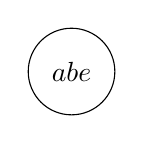
\begin{tikzpicture} \draw (0,0) circle (0.55cm) node at (0,0) {$abe$}; \end{tikzpicture}}\,+abf-a^2e\,\raisebox{-4.5mm}{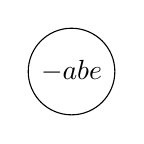
\begin{tikzpicture} \draw (0,0) circle (0.55cm) node at (0,0) {$-abe$}; \end{tikzpicture}}}{a+b}
%%%
seu $\displaystyle\frac{b}{a+b}\,\smallfrown\,bf-ae$. 
%
\pend \pstart\noindent
\rule[0cm]{0mm}{24pt}$bf,\;-\displaystyle\frac{ab}{a+b}\,\smallfrown\,e+f \,\sqcap\,\displaystyle\frac{\ovalbox{$abf$}\;+b^2f-abe\;\ovalbox{$-abf$}}{a+b}\,\sqcap\,\displaystyle\frac{b}{a+b}\; \overline{bf-ae}$.%
$\rule[-4mm]{0mm}{10mm}$
%%%
%%% \raisebox{-4.5mm}{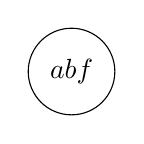
\begin{tikzpicture} \draw (0,0) circle (0.55cm) node at (0,0) {$abf$}; \end{tikzpicture}}\,+b^2f-abe\,\raisebox{-4.5mm}{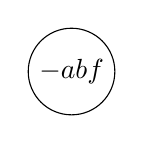
\begin{tikzpicture} \draw (0,0) circle (0.55cm) node at (0,0) {$-abf$}; \end{tikzpicture}}
%%%
%
%%
\pend
%
\pstart
\rule[0cm]{0mm}{10pt}\edtext{Ergo differentiae}{\lemma{Ergo}\Bfootnote{\textit{(1)}~potentia \textit{(2)}~differentia \textit{(3)}~differentiae~\textit{L}}} 
inter 
\edtext{dimidiam}{\lemma{}\Bfootnote{dimidiam \textit{erg.}~\textit{L}}} 
potentiam\protect\index{Sachverzeichnis}{potentia ictus} 
\edtext{ictus et}{\lemma{ictus}\Bfootnote{\textit{(1)}~est corporis \textit{(2)}~et~\textit{L}}} 
totam corporis%
\protect\index{Sachverzeichnis}{potentia tota corporis}
sunt inter se in ratione corporum. Quoniam autem tota minoris potentia\protect\index{Sachverzeichnis}{potentia}
absorbetur, et in majori \textit{bf} restat
%
$\displaystyle\frac{b}{a+b}\;\overline{bf-ae}$.%
$\rule[-4mm]{0mm}{10mm}$
%
\pend \pstart
Sed jam video in calculo oriri difficultatem. Nimirum 
%
\edtext{cum residua}{%
\lemma{cum}%
\Bfootnote{%
\textit{(1)}~residuum %
\textit{(2)}~residua%
~\textit{L}%
}}
%
potentia\protect\index{Sachverzeichnis}{potentia}
in corporibus post potentiam ictus\protect\index{Sachverzeichnis}{potentia ictus} subtractam sit
$\displaystyle\frac{b-a}{a+b}\,\smallfrown\,bf-ae$.
Hinc patet
si sit 
$bf\,\groesser\,ae$,
debere et esse 
$b\,\groesser\,a$.
\rule[0cm]{0mm}{10pt}\edtext{Alioqui haec}{\lemma{Alioqui}\Bfootnote{\textit{(1)}~erit \textit{(2)}~haec~\textit{L}}}
%
residua potentia\protect\index{Sachverzeichnis}{potentia}
erit quantitas negativa, seu vis ictus\protect\index{Sachverzeichnis}{vis ictus} erit major  
\edtext{quam potentia\protect\index{Sachverzeichnis}{potentia} corporum,}{\lemma{quam potentia}\Bfootnote{\textit{(1)}~corporis \textit{(2)}~corporum,~\textit{L}}}
quod est absurdum, 
%
\edlabel{37_05_157-158_3a}unde patet cum corpus
\edtext{potentius est minus tunc}{\lemma{potentius}\Bfootnote{\textit{(1)}~minus est \textit{(2)}~est minus~\textit{L}}} 
regulam
%
\edtext{de eadem}{\lemma{de}\Bfootnote{\textit{(1)}~ictus \textit{(2)}~eadem~\textit{L}}} 
ictus potentia%
\protect\index{Sachverzeichnis}{potentia ictus} eadem existente celeritate appropinquationis%
\protect\index{Sachverzeichnis}{celeritas appropinquationis}
in corporibus concurrentibus esse falsam.\edlabel{37_05_157-158_3b}
\pend \pstart
Quod si sic ratiocinemur, potentiae\protect\index{Sachverzeichnis}{potentia} debilioris aequalem potentiam\protect\index{Sachverzeichnis}{potentia} opponendam esse a fortiori detractam, sed et hoc absurdum est,
\edtext{quia nulla}{\lemma{quia}\Bfootnote{\textit{(1)}~tunc nullus \textit{(2)}~nulla~\textit{L}}} 
%
erit vis ictus,%
\protect\index{Sachverzeichnis}{vis ictus} si corpus motum incurrat in quiescens%
\protect\index{Sachverzeichnis}{corpus quiescens}
%
%
\edlabel{37_05_157-158_4a}%
\edtext{}{% NEUER ABSATZ UND VARIANTEN – "quantumcumque"
{\xxref%
{37_05_157-158_4a}{37_05_157-158_4b}}%
\lemma{quantumcumque.}%
\Bfootnote{%
\textit{(1)}~Redeamus ad navim\protect\index{Sachverzeichnis}{navis} nostram, et ita tantum instituamus calculum ut potentia\protect\index{Sachverzeichnis}{potentia} sit salva. \textit{(2)}~An~\textit{L}}}%
quantumcumque.
\pend
%
\pstart
An%
\edlabel{37_05_157-158_4b}
%
dicemus vim ictus\protect\index{Sachverzeichnis}{vis ictus} semper tantam esse, ut
utrumque corpus dimidiam itineris partem conficere intelligatur. Sed nec hoc
fingi potest, nam si unum corpus sit valde magnum, si hoc poneremus dimidiam 
itineris partem conficere, mirifice augeretur potentia\protect\index{Sachverzeichnis}{potentia}. 
%
%
\edlabel{37_05_157-158_5a}%
\edtext{}{% C-Footnote
{\xxref%
{37_05_157-158_5a}{37_05_157-158_5b}}%
\lemma{Quod \lbrack...\rbrack\ navis}%
\Cfootnote{%
Siehe die ausführliche Behandlung des Stoßes anhand der Schiffsanalogie im ebenfalls auf den 10.\ (20.) Juni 1677 datierten Konzept N.~\ref{57269}.}}%
%
Quod si ergo vim ictus\protect\index{Sachverzeichnis}{vis ictus} faciamus 
%
qualem requirit navis\protect\index{Sachverzeichnis}{navis},\edlabel{37_05_157-158_5b}
%
tunc semper utique
major erit potentia
\edtext{tota\protect\index{Sachverzeichnis}{potentia tota}}{\lemma{tota}\Bfootnote{\textit{erg. L}}}
%
\edtext{quam vis}{\lemma{}\Bfootnote{vis \textit{erg. L}}} 
%
ictus\protect\index{Sachverzeichnis}{vis ictus}.
Nam
%
%%%%%%%%%%%%%%%%%%%%%%%%%%%%%%%
%%%
%%% === end of fol. 158 r ===
%%%
%%% === fol. 158 v ===
%%%
%%%%%%%%%%%%%%%%%%%%%%%%%%%%%%%%%
%
\lbrack158~v\textsuperscript{o}\rbrack\
%
si sit:
\pend 
%
\vspace{2.5em} %%%%%%%%% Diagramm 2
\centerline{%
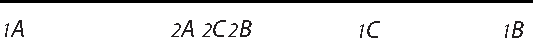
\includegraphics[width=0.66\textwidth]{%
gesamttex/edit_VIII,3/images/LH_37_05_157-158_d2_158v.pdf%
}} 
\vspace{0.5em}
\centerline{%
\lbrack\textit{Fig.~2}\rbrack%
}
% \newpage%
\vspace{1.5em}
%
\pstart\noindent 
\edtext{potentia ictus\protect\index{Sachverzeichnis}{potentia ictus}:}{%
\lemma{}%
\Afootnote{%
\textit{Neben} potentia ictus, \textit{gestrichen:} %
{\footnotesize $\dfrac{\leibdashv ae \leibvdash bf}{a+b} \,\sqcap\, {\scriptstyle 1}C{\scriptstyle 2}C$}%
}}
%
%
2\textit{abl}, et $l\,\sqcap\,\displaystyle\frac{e+f}{a+b}$. 
Ergo potentia ictus\protect\index{Sachverzeichnis}{potentia ictus} $\displaystyle\frac{2ab}{a+b}\,\smallfrown\,e+f$, eadem scilicet quae ante. 
%
\rule[0cm]{0mm}{18pt}Nimirum $\begin{array}{c}
    {\scriptstyle 1}A{\scriptstyle 1}C\,\sqcap\,bl \\ 
    {\scriptstyle 1}B{\scriptstyle 1}C\,\sqcap\,al \\ 
\end{array}$.
%
Celeritas corporis \textit{A} debet fingi 
%
\edtext{\textit{bl}, et potentia\protect\index{Sachverzeichnis}{potentia}}{\lemma{\textit{bl},}\Bfootnote{\textit{(1)}~nempe \textit{(2)}~et~\textit{L}}} 
%
ejus 
%
\edtext{erit \textit{abl}. Celeritas corporis}{\lemma{erit \textit{abl}}\Bfootnote{\textit{(1)}~, celeritas corporis \textit{(2)}~. Celeritas corporis~\textit{L}}} 
%
\rule[0cm]{0mm}{10pt}\textit{B} debet esse \textit{al}, et potentia\protect\index{Sachverzeichnis}{potentia} erit etiam \textit{abl}. Ergo potentia \makebox[1.0\textwidth][s]{ictus\protect\index{Sachverzeichnis}{potentia ictus} erit
$\displaystyle\frac{2ab}{a+b}\smallfrown\,\overline{e+f}$. Videndum an haec potentia ictus\protect\index{Sachverzeichnis}{potentia ictus} aliquando sit
major quam} 
\pend
\newpage
\pstart
\noindent  potentia\protect\index{Sachverzeichnis}{potentia tota} corporum tota
$ae+bf-\overline{\displaystyle\frac{2ab}{a+b}\overline{e+f}}$. 
%
Ergo 
$\displaystyle\frac{a^2e+abf+bae+b^2f-2abe-2abf}{a+b}$
$\,\sqcap\,\displaystyle\frac{+a^2e-abe+b^2f-abf}{a+b}\,\sqcap\,$ $\displaystyle\frac{a-b\smallfrown ae,,\;+b-a\smallfrown bf}{a+b}$.\rule[0cm]{0mm}{18pt}
%
\pend
%
\pstart\noindent
Seu
$\displaystyle\frac{a-b}{a+b}\,\smallfrown\,\overline{ae-bf}$
ut ante.\rule[0cm]{0mm}{18pt}
%
\edtext{Unde patet}{\lemma{Unde}\Bfootnote{\textit{(1)}~fiet \textit{(2)}~patet~\textit{L}}} 
%
calculum utrumque\lbrack,\rbrack\
de supposita eadem potentia ictus\protect\index{Sachverzeichnis}{potentia ictus}, quando eadem
\rule[0cm]{0mm}{10pt}corpora eadem celeritate sibi accedunt, et de navi\protect\index{Sachverzeichnis}{navis}, coincidere. 
\edtext{Illud hic obiter noto\lbrack:\rbrack}{%
\lemma{}%
\Afootnote{\textit{Am Rand:}\ NB}}
%
\rule[0cm]{0mm}{16pt}quantitatem $\displaystyle\frac{a-b}{a+b}\,\smallfrown\,\overline{ae-bf}$
videri diversimodo se
%
\edtext{habere ad $a\cdot e$  quam ad $b\cdot f$. Quod}{\lemma{habere ad}\Bfootnote{%
\textit{(1)}~\textit{a} quam ad \textit{b} et ad \textit{e} quam ad \textit{f}. %
\textit{(2)}~$a\cdot e$ \lbrack...\rbrack\ $b\cdot f$. Quod~\textit{L}}}
%
\rule[0cm]{0mm}{10pt}tamen non est, ut apparet si
\rule[-0.2cm]{0mm}{16pt}absolvatur multiplicatio, nam patet esse
$\displaystyle\frac{\begin{array}{c}a^2e-abe \\ b^2f-abf \end{array}}{a+b}$.%
$\rule[-4mm]{0mm}{10mm}$
%
\pend
%
\pstart
Potentia%
\protect\index{Sachverzeichnis}{potentia ictus} ictus illa est qua corpora duo Elastica%
\protect\index{Sachverzeichnis}{corpus elasticum} concurrentia flectentur. Impossibile
est autem plus esse potentiae%
\protect\index{Sachverzeichnis}{potentia} in ictu, quam in ambobus corporibus simul ante ictum\protect\index{Sachverzeichnis}{ictus}. Ictus\protect\index{Sachverzeichnis}{ictus}
enim utique effectus est potentiae\protect\index{Sachverzeichnis}{potentia} corporum. Videtur corpus corpori obstanti ictum\protect\index{Sachverzeichnis}{ictus}
infligere, in quantum ei obstat. Si corpus in aliquod corpus incurrat, idque sit quiescens,%
\protect\index{Sachverzeichnis}{corpus quiescens}
obstaculum in eo consistit, quod pergere non potest eadem qua ante celeritate, sed ejus celeritas,
%
\edtext{diminuitur. Ergo}{\lemma{diminuitur.}\Bfootnote{\textit{(1)}~Ergo corpus impingens potentiam\protect\index{Sachverzeichnis}{potentia} tantam amittit, quantam alteri quiescenti tribuit \textit{(2)}~Ergo~\textit{L}}} 
%
tantus est ictus\protect\index{Sachverzeichnis}{ictus} quanta est potentiae\protect\index{Sachverzeichnis}{potentia}  mutatio\protect\index{Sachverzeichnis}{mutatio potentiae}.%
\pend
%
\pstart
\edtext{Atque hoc quidem dignum est, ut \edtext{peculiari scheda}{\lemma{peculiari \lbrack...\rbrack\ \textit{ictus}}\Cfootnote{Siehe N.~\ref{57271}.}} tractetur \textit{De vi ictus}\protect\index{Sachverzeichnis}{vis ictus}.}{%
\lemma{}%
\Bfootnote{%
Atque \lbrack...\rbrack\  \textit{ictus}. %
\textit{erg.\ L}%
}}
\pend
\count\Bfootins=1200%
\count\Afootins=1200%
\count\Cfootins=1200
%
%
